\documentclass{article}
\usepackage[utf8]{inputenc}
\usepackage[spanish]{babel}
\usepackage{graphicx}
\usepackage{geometry}
\usepackage{enumerate}
\usepackage{titlesec}
\usepackage{float}
\usepackage{amsmath}

\geometry{letterpaper, margin = 1.5cm}

%Datos de la Portada
\title{Herrramientas Computacionales \\ Practica 2}
\author{Medina Martinez Jonathan Jason \\ 2023640061}
\date{7 de marzo de 2023}

\begin{document} %Inicio del Documento

\fontsize{12}{14}\selectfont

\begin{figure}[t] %Logos Portada


\includegraphics[width=2.5 cm]{Logo1.jpeg}
\hfill

\includegraphics[width=3 cm]{Logo2.png}

\end{figure}

\maketitle %Titulo Portada
\newpage

\tableofcontents %Indice
\newpage

\section{Objetivo}

Realizar operaciones con diferentes tipos de operadores y funciones basicas.

\section{Introducción}

En esta practica se realizaran operaciones en el command window de MATLAB con distintos tipos de operadores y Funciones basicas como :
\begin{enumerate}
    \item \textbf{nthroot}
    \item \textbf{sqrt}
    \item \textbf{log}
    \item entre otras
\end{enumerate}

Ademas de emplear algunas propiedades de los logarimos naturales.

\newpage

\section{Desarrollo}

Utilizando el Command Window de MATLAB, resuelva las siguientes operaciones.

\begin{enumerate}
    \item 
    \
    \begin{figure}[H]
    \centering
    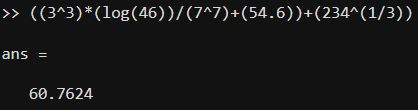
\includegraphics[height=3cm]{img1.jpg}
    \end{figure}

    \item 
    \
    \begin{figure}[H]
    \centering
    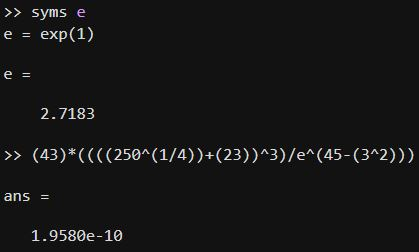
\includegraphics[height=6cm]{img2.jpg}
    \end{figure}

    \item 
    \
    \begin{figure}[H]
    \centering
    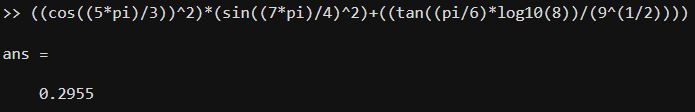
\includegraphics[height=2.5cm]{img3.jpg}
    \end{figure}

    \item 
    \
    \begin{figure}[H]
    \centering
    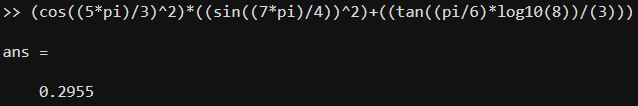
\includegraphics[height=3cm]{img4.jpg}
    \end{figure}
    
    \newpage
    
    \item 

    Sea x = 10.5, calcule:

    \begin{enumerate}[a)]

        \item 
        \
        \begin{figure}[H]
        \centering
        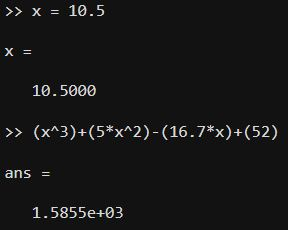
\includegraphics[height=6cm]{img5a.jpg}
        \end{figure}

        \item 
        \
        \begin{figure}[H]
        \centering
        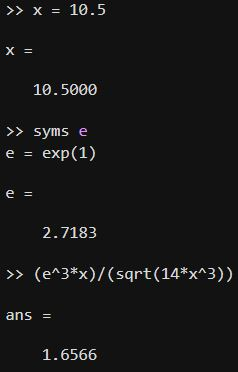
\includegraphics[height=6cm]{img5b.jpg}
        \end{figure}

        \item 
        \
        \begin{figure}[H]
        \centering
        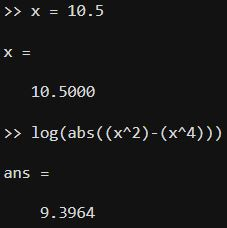
\includegraphics[height=6cm]{img5c.jpg}
        \end{figure}

    \end{enumerate}
    
    \newpage
    
    \item 

    Sea x = 19.6 y z = 7.8, calcule:

    \begin{enumerate}[a)]

        \item 
        \
        \begin{figure}[H]
        \centering
        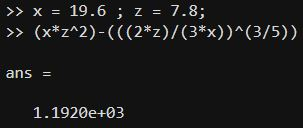
\includegraphics[height=6cm]{img6a.jpg}
        \end{figure}

        \item 
        \
        \begin{figure}[H]
        \centering
        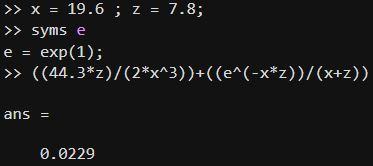
\includegraphics[height=6cm]{img6b.jpg}
        \end{figure}

    \end{enumerate}
    
    \item 

    Sea a=14.32, b=6.18, c=\text{-}6.25 y d=3.5(ab\text{-}c), calcule:

    \begin{enumerate}[a)]

        \item
        \
        \begin{figure}[H]
        \centering
        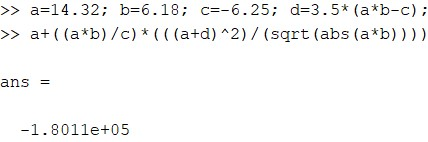
\includegraphics[height=5cm]{img7a.jpg}
        \end{figure}
        \newpage
        \item 
        \
        \begin{figure}[H]
        \centering
        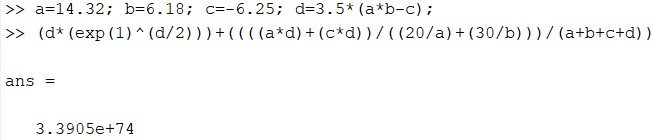
\includegraphics[width=18cm]{img7b.jpg}
        \end{figure}

    \end{enumerate}

    \item 

    Encuentre la raız cubica de \text{-}27, tanto con la funcion \textbf{ntroot} como con elevar \text{-}27 a la potencia 1/3. Explique la diferencia en sus respuestas. Pruebe que ambos resultados de hecho son respuestas correctas al elevarlos al cubo y mostrar que son iguales a \text{-}27.
    
    \begin{figure}[H]
    \centering
    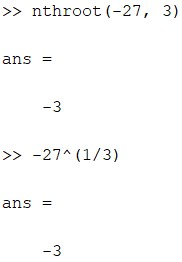
\includegraphics[height=8cm]{img8.jpg}
    \end{figure}

    En ambos casos, obtenemos la misma respuesta "-3", que es la raiz cubica de -27. La diferencia en los resultados se debe a que la función "nthroot" utiliza un algoritmo especifico para encontrar raices n-esimas, mientras que elevar un numero a una potencia fraccionaria es una operacion matematica estandar. Sin embargo, ambos resultados son correctos y dan la misma respuesta cuando se elevan al cubo y se comprueba que son iguales a -27.

    \newpage
    \item 

    MATLAB contiene funciones para calcular el logaritmo natural (log), el logaritmo base 10 (log10) y el logaritmo base 2 (log2). Sin embargo, si quiere encontrar un logaritmo de base distinta (por ejemplo, base b), tendra que aplicar la siguinete formula:
    
    \centering 
    \begin{equation*}
        \log_{b}(x) = \frac{\ln(x)}{\ln(b)}
    \end{equation*}

    
    ¿Cual es el log\textsubscript{1}, lo\textsubscript{2}, log\textsubscript{3}, log\textsubscript{4}, log\textsubscript{5}, log\textsubscript{6}, log\textsubscript{7}, log\textsubscript{8}, log\textsubscript{9} y log\textsubscript{10} de 10?
    
    \begin{figure}[H]
    \centering
    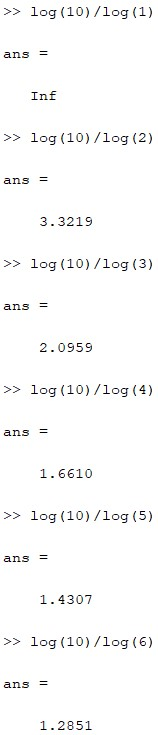
\includegraphics[width=4cm]{img9a.jpg}
    \end{figure}
    \begin{figure}[H]
    \centering
    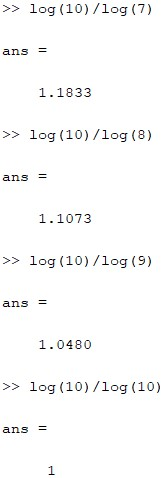
\includegraphics[width=4cm]{img9b.jpg}
    \end{figure}

    \item 

    La distancia $d$ de un punto $(x0, y0)$ a una recta $Ax + By + C = 0$ viene dada por:
    
    $$d = \frac{|Ax_0 + By_0 + C|}{\sqrt{A^2 + B^2}}$$
    
    Determine la distancia del punto $(4,−7)$ a la recta $2x+15y−13 = 0$.
    
    Primero determine las variables $A, B, C, x0, y0$ y despues calcule $d$.
    
    \begin{figure}[H]
    \centering
    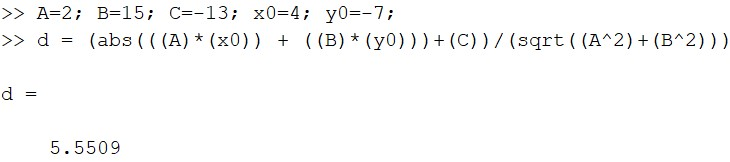
\includegraphics[height=4cm]{img10.jpg}
    \end{figure}

\end{enumerate}

\newpage

\section{Conclusion}

Los operadores en MATLAB nos permite realizar operaciones de forma mas sencilla y rapida al ahorrarnos procesos que normalmente se podrian volver complejos o redundantes. 

\end{document}